This chapter reports what the five dual-stream detectors achieved. Each detector was trained twice, once on the RGB annotations and once on the SAR annotations (Section~\ref{sec:implementation_of_selected_design}), so there are ten runs in total. For each run, the checkpoint was picked on the selection split. MOS-Ship~\cite{you2026multi} has no official test split, so we use its val split of 500 tiles (250 clean and 250 cloud) as the test set. Every score in this chapter comes from that set. Section~\ref{sec:performance_evaluation} gives the results and picks the best model. Section~\ref{sec:analysis_of_design_solutions} looks at why the models behave the way they do, and Section~\ref{sec:discussion} discusses what this means for the research.

\section{Performance Evaluation}
\label{sec:performance_evaluation}
Our main metric is mAP50:95. It averages the mean average precision (mAP) over ten IoU thresholds, from 0.50 to 0.95 in steps of 0.05, so a model only scores high if its boxes fit each ship tightly. We also report mAP50 and mAP75, which use a single IoU threshold of 0.5 and 0.75. All three use rotated IoU, except for Faster R-CNN~\cite{7485869}, as explained below. Precision, recall and F1 are measured at one fixed score threshold, the one that gave the best F1 on the selection split, with a detection counted as correct at IoU 0.5. Since this threshold was chosen before the test, these numbers show how the model would behave in real use. Speed is given in frames per second (FPS) for one 1024 × 1024 tile at batch size 1.

\subsection{Evaluation Metrics}

\paragraph{IoU.}
Intersection over Union measures the overlap between a predicted box
$B_p$ and a ground-truth box $B_{gt}$:
\begin{equation}
\mathrm{IoU} = \frac{\mathrm{area}(B_p \cap B_{gt})}{\mathrm{area}(B_p \cup B_{gt})}
\end{equation}
Rotated IoU is used for all models except Faster R-CNN~\cite{7485869}, which predicts
horizontal boxes.\\

\paragraph{Precision, Recall and F1.}
A prediction is a true positive (TP) if its IoU with an unmatched
ground-truth box meets the threshold. Otherwise it is a false positive
(FP). Unmatched ground-truth boxes are false negatives (FN).\\
\begin{equation}
P = \frac{TP}{TP+FP}, \qquad
R = \frac{TP}{TP+FN}, \qquad
F1 = \frac{2PR}{P+R}
\end{equation}
Precision is the share of predictions that are correct. Recall is the
share of ships that are detected. F1 is their harmonic mean.\\

\paragraph{AP and mAP.}
AP is the area under the precision--recall curve. mAP is the mean AP
across classes. The dataset has a single class, so mAP equals AP.
mAP50 and mAP75 use IoU thresholds of 0.50 and 0.75. mAP50:95 averages
AP over ten IoU thresholds from 0.50 to 0.95 in steps of 0.05.\\

\paragraph{Evaluation Settings.}
mAP50:95 is the main metric. It calculates the mean average precision (mAP) across 10 IoU thresholds, ranging from 0.50 to 0.95 with steps of 0.05, which means that the model must fit the boxes around each ship closely in order to achieve a high score. mAP50 and mAP75 also reported using a single IoU threshold of 0.5 and 0.75 respectively. Except for Faster R-CNN~\cite{7485869}, all three utilize rotated IoU, which is explained below. Precision, recall and F1 are calculated at a single fixed score threshold (the one that produced the best F1 on the selection split), where a detection is considered correct if the IoU is 0.5. These numbers give an indication of how the model would behave in real use, as this threshold was selected prior to the test. Speed is given in frames per second (FPS) for one 1024 × 1024 tile at batch size 1.

\subsection{Results with RGB Annotations}

% \newlength{\tw}  % uncomment ONLY if \tw is not already defined elsewhere in your file

\begin{table}[htbp]
\centering
\footnotesize
\renewcommand{\arraystretch}{1.5}
\setlength{\tabcolsep}{3pt}
\setlength{\tw}{\dimexpr\textwidth-20\tabcolsep-11\arrayrulewidth\relax}

\begin{tabular}{
|>{\raggedright\arraybackslash}p{0.16\tw}
|>{\centering\arraybackslash}p{0.09\tw}
|>{\centering\arraybackslash}p{0.10\tw}
|>{\centering\arraybackslash}p{0.10\tw}
|>{\centering\arraybackslash}p{0.12\tw}
|>{\centering\arraybackslash}p{0.13\tw}
|>{\centering\arraybackslash}p{0.10\tw}
|>{\centering\arraybackslash}p{0.07\tw}
|>{\centering\arraybackslash}p{0.06\tw}
|>{\centering\arraybackslash}p{0.07\tw}|
}
\hline
\rowcolor{gray!20}
\textbf{Model} &
\textbf{Best epoch} &
\textbf{mAP50} &
\textbf{mAP75} &
\textbf{mAP50:95} &
\textbf{Precision} &
\textbf{Recall} &
\textbf{F1} &
\textbf{FP} &
\textbf{FN} \\
\hline

YOLO26-OBB &
19 &
0.994 &
\textbf{0.989} &
\textbf{0.871} &
0.983 &
0.981 &
\textbf{0.982} &
19 &
21 \\
\hline

Oriented R-CNN\cite{xie2021oriented} &
21 &
0.992 &
0.985 &
0.854 &
0.981 &
0.982 &
0.981 &
21 &
20 \\
\hline

Oriented- Former &
18 &
0.993 &
0.983 &
0.840 &
0.982 &
0.961 &
0.971 &
19 &
43 \\
\hline

S2A-Net &
22 &
\textbf{0.995} &
0.934 &
0.734 &
0.973 &
\textbf{0.987} &
0.980 &
30 &
\textbf{14} \\
\hline

Faster R-CNN$^{*}$ &
18 &
0.987 &
0.917 &
0.857 &
\textbf{0.996} &
0.961 &
0.978 &
\textbf{4} &
43 \\
\hline
\end{tabular}


\caption{Test results with RGB annotations (1098 ground-truth boxes)}
\label{tab:rgb_results}
\end{table}


The five detectors trained and tested on the RGB labels are shown in Table ~\ref{tab:rgb_results}. They are almost equal at IoU 0.5. mAP50 is relatively high (between 0.987 and 0.995), meaning that almost all ships are detected by all models. It is the more stringent metrics that separate the models. YOLO26-OBB~\cite{jocher2026ultralytics} has the best mAP50:95 at 0.871, followed by Oriented R-CNN (0.854) and OrientedFormer~\cite{zhao2024orientedformer} (0.840).\\

S2A-Net~\cite{han2021align} shows a mixed result. It achieves the highest mAP50 (0.995) and the highest recall (0.987) of all models. However, its mAP75 falls to 0.934 and its mAP50:95 to 0.734. This indicates that S2A-Net detects nearly all ships, but its predicted boxes are less tightly aligned with the ground truth than those of the other models. OrientedFormer~\cite{zhao2024orientedformer} misses the most ships. It produces 43 false negatives, compared with 20 for Oriented R-CNN and 21 for YOLO26-OBB~\cite{jocher2026ultralytics}. This explains its lower recall of 0.961.

Faster R-CNN~\cite{7485869} is very close to the top with a mAP50:95 of 0.857 and 4 false positives. That number isn't directly comparable, though. It is based on horizontal IoU with the outer box of each ship, which is more tolerant. If its boxes are also scored with rotated IoU, as the other four, then its mAP50 drops to 0.093. Section 5.2 tells the why.

\subsection{Results with SAR Annotations}


\begin{table}[htbp]
\centering

\resizebox{\textwidth}{!}{%
\begin{tabular}{|l|c|c|c|c|c|c|c|c|c|}
\hline
\textbf{Model} & \textbf{Best epoch} & \textbf{mAP50} & \textbf{mAP75} & \textbf{mAP50:95} & \textbf{Precision} & \textbf{Recall} & \textbf{F1} & \textbf{FP} & \textbf{FN} \\
\hline
YOLO26-OBB     & 12 & 0.931          & \textbf{0.680} & \textbf{0.579} & 0.893          & 0.908          & 0.901          & 116         & 98          \\
Oriented R-CNN\cite{xie2021oriented} & 10 & 0.859          & 0.461          & 0.454          & 0.857          & 0.850          & 0.854          & 151         & 160         \\
OrientedFormer & 12 & 0.847          & 0.385          & 0.430          & 0.808          & 0.791          & 0.799          & 201         & 223         \\
S2A-Net        & 14 & 0.780          & 0.062          & 0.274          & 0.833          & 0.792          & 0.812          & 169         & 222         \\
Faster R-CNN*  & 6  & \textbf{0.953} & 0.559          & 0.558          & \textbf{0.925} & \textbf{0.916} & \textbf{0.920} & \textbf{79} & \textbf{90} \\
\hline
\end{tabular}%
}

\vspace{4pt}
\caption{Test results with SAR annotations (1068 ground-truth boxes)}
\label{tab:sar_results}
\end{table}

Table~\ref{tab:sar_results} repeats the test with the SAR labels. The test set now has 1068 boxes instead of 1098, because the SAR annotators marked a slightly different set of ships. Every model scores lower. mAP50 drops to between 0.780 and 0.953, and the drop gets much bigger at stricter IoU. mAP75, which was about 0.98 for most models, falls to between 0.062 and 0.680. False positives also rise, from 4 to 30 per model to between 79 and 201. \\

The order of the oriented models stays the same. YOLO26-OBB~\cite{jocher2026ultralytics} is still first (mAP50:95 0.579), then Oriented R-CNN (0.454), OrientedFormer~\cite{zhao2024orientedformer} (0.430) and S2A-Net~\cite{han2021align} (0.274). S2A-Net~\cite{han2021align} suffers most at strict IoU, with a mAP75 of only 0.062. Figure 5.1 puts both label sources side by side.\\

% ******** SAR vs RGB annotation bar plot*******\\

\begin{figure}[htbp]
\centering
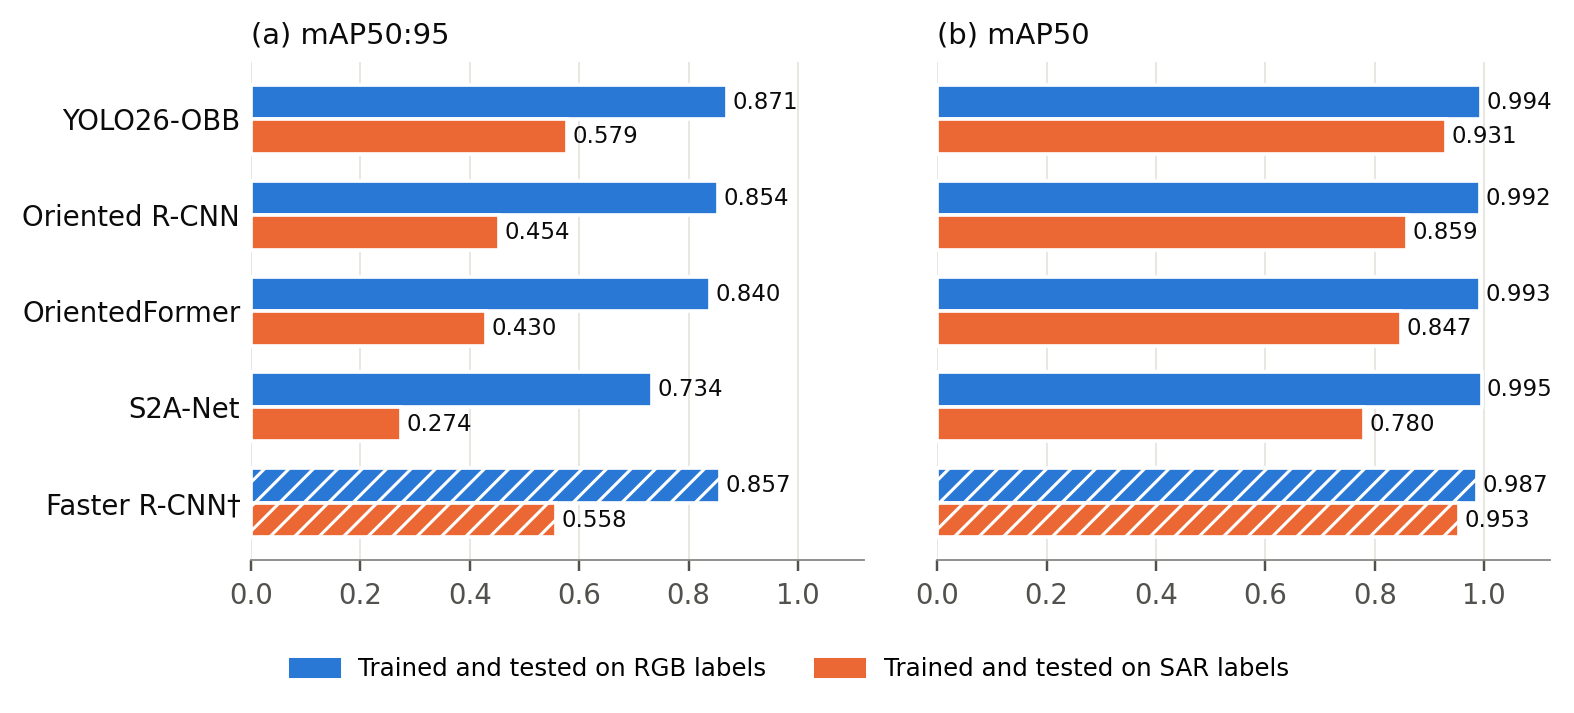
\includegraphics[width=1\textwidth]{images/rgb_vs_sar_labels.png}
\caption{Detection performance with RGB and SAR annotations.}
\label{fig:sar_vs_rgb_lables}
\end{figure}
\\
Figure~\ref{fig:sar_vs_rgb_lables}: Test mAP50:95 (a) and mAP50 (b) for each detector, trained and tested on RGB labels (blue) or SAR labels (orange). *Faster R-CNN~\cite{7485869} (hatched) is scored with horizontal IoU.
\\

\newpage
\subsection{Clean and Cloud Tiles}
\\
\begin{table}[htbp]
\centering

\begin{tabular}{|l|c|c|c|c|c|c|}
\hline
 & \multicolumn{3}{c|}{\textbf{RGB annotations}} & \multicolumn{3}{c|}{\textbf{SAR annotations}} \\
\cline{2-7}
\textbf{Model} & \textbf{Clean} & \textbf{Cloud} & \textbf{Drop(\%)} & \textbf{Clean} & \textbf{Cloud} & \textbf{Drop(\%)} \\
\hline
YOLO26-OBB     & \textbf{0.873} & \textbf{0.870} & \textbf{0.3} & \textbf{0.583} & \textbf{0.576} & 0.7          \\
Oriented R-CNN\cite{xie2021oriented} & 0.862          & 0.846          & 1.5          & 0.457          & 0.453          & 0.4          \\
OrientedFormer & 0.844          & 0.836          & 0.8          & 0.436          & 0.425          & 1.0          \\
S2A-Net        & 0.739          & 0.729          & 0.9          & 0.278          & 0.272          & 0.6          \\
Faster R-CNN*  & 0.861          & 0.854          & 0.7          & 0.560          & 0.557          & \textbf{0.2} \\
\hline
\end{tabular}
\vspace{4pt}
\caption{mAP50:95 on clean and cloud tiles (drop in points)}
\label{tab:cloud_drop}
\end{table}

\\

The test set has 250 clean tiles and the same 250 tiles with synthetic clouds. Table~\ref{tab:cloud_drop} breaks down mAP50:95 into these two groups. Cloud is extremely cheap. The maximum decrease is 1.5\%(Oriented R-CNN with RGB labels) and for YOLO26-OBB~\cite{jocher2026ultralytics} it is 0.3\%. None of the models lose more than 1.0\% with SAR labels. Thus, the official cloud tiles are not tough enough to split the models. We come back to this in Section 5.2.

\subsection{Model Size and Speed}
\\

\begin{table}[htbp]
\centering

\begin{tabular}{|l|c|c|c|c|c|}
\hline
 & & \multicolumn{2}{c|}{\textbf{RGB-label run}} & \multicolumn{2}{c|}{\textbf{SAR-label run}} \\
\cline{3-6}
\textbf{Model} & \textbf{Params (M)} & \textbf{FPS} & \textbf{GPU} & \textbf{FPS} & \textbf{GPU} \\
\hline
YOLO26-OBB     & \textbf{33.2} & \textbf{24.7} & RTX 3070    & \textbf{24.9} & RTX 3070    \\
Oriented R-CNN & 75.9          & 5.9           & RTX 3070    & 12.1          & RTX 3070 Ti \\
OrientedFormer & 79.3          & 8.0           & RTX 3070 Ti & 8.1           & RTX 3070 Ti \\
S2A-Net        & 73.2          & 12.7          & RTX 3070 Ti & 12.9          & RTX 3070 Ti \\
Faster R-CNN*  & 75.9          & 14.7          & RTX 3070 Ti & 11.5          & RTX 3070    \\
\hline
\end{tabular}
\vspace{4pt}
\caption{Model size and inference speed ($1024 \times 1024$ tile, batch size 1)}
\label{tab:model_speed_overview}
\end{table}
\\
Table~\ref{tab:model_speed_overview} compares the size and speed of each model. YOLO26-OBB~\cite{jocher2026ultralytics} is the smallest model with 33.2 M parameters, which is less than half of the other ones. It's also the fastest, running at approximately 25 FPS in both runs. The other FPS numbers require care. They were tested on two different GPUs, and the same Oriented R-CNN\cite{xie2021oriented} performed at 5.9 FPS and 12.1 FPS. We only believe the general picture. YOLO26-OBB~\cite{jocher2026ultralytics} is by far the fastest, and none of the other models achieve a speed of more than 15 FPS.\\

The selection of the Best Performing Model is based on the following criteria:\\

Models were ranked based on four criteria, in order of importance:
\begin{itemize}
    \item \textbf{Accuracy with RGB labels:} YOLO26-OBB~\cite{jocher2026ultralytics} has the highest mAP$_{50:95}$ (0.871).
    \item \textbf{Accuracy with SAR labels:} YOLO26-OBB~\cite{jocher2026ultralytics} is again the top oriented model (0.579).
    \item \textbf{Behaviour at a fixed threshold:} Its F1 of 0.982 is the highest, just ahead of Oriented R-CNN (0.981).
    \item \textbf{Cost:} It has the fewest parameters and the highest FPS.
\end{itemize}

On all the criteria, YOLO26-OBB~\cite{jocher2026ultralytics} is the best performing model, hence it is chosen as the best model and the base for the next phase. The best of the four models that start from ImageNet weights is oriented R-CNN\cite{xie2021oriented}, which is a close second on accuracy. One caveat applies. YOLO26-OBB~\cite{jocher2026ultralytics} is based on a detector pretrained on DOTAv1\cite{xia2018dota}, which contains ships viewed from above, and the other four only receive an ImageNet backbone. This head start may be a source of its lead. It is predicting on two of the most dense test tiles as shown in figure~\ref{fig:yolo_samples}.\\ 

\begin{figure}[htbp]
\centering
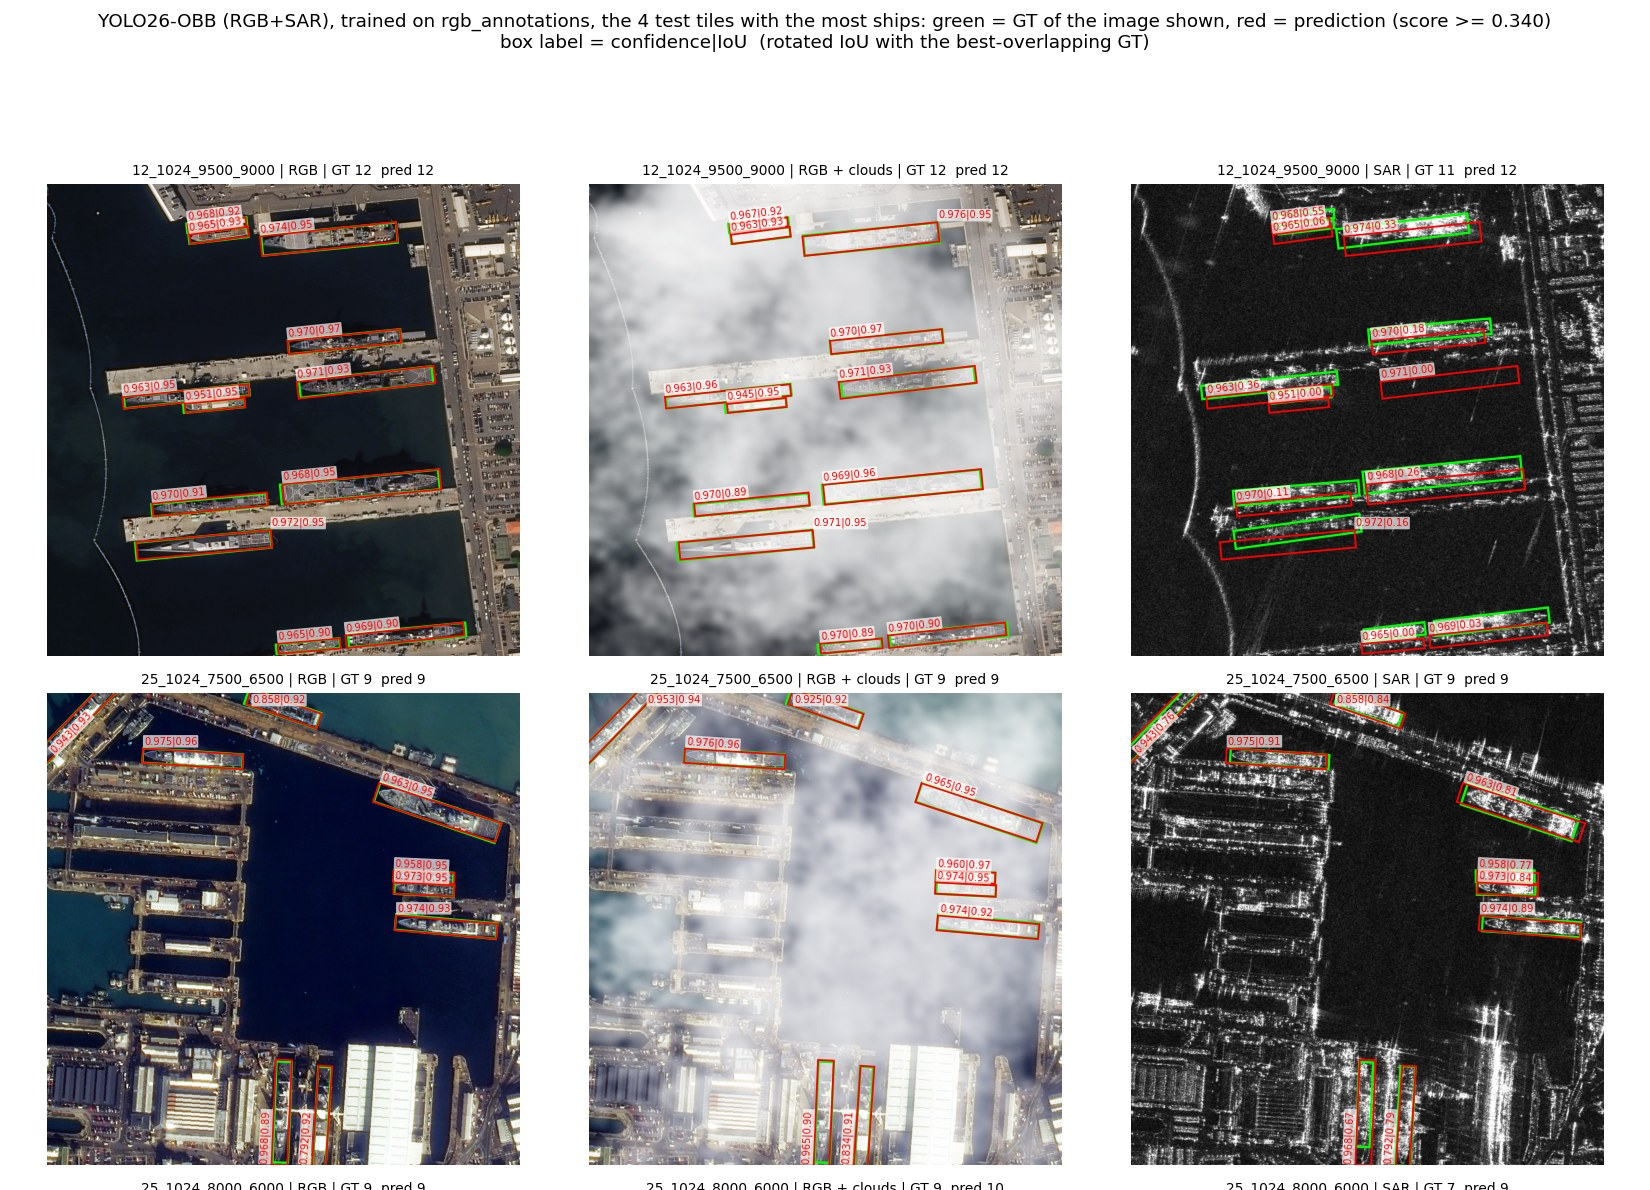
\includegraphics[width=1\textwidth]{images/yolo_samples.jpg}
\caption{Sample detections of YOLO26-OBB.}
\label{fig:yolo_samples}
\end{figure}

Figure~\ref{fig:yolo_samples} shows YOLO26-OBB (RGB labels) on two of the test tiles with the highest number of ships. The RGB tile, cloud copy and the SAR tile are shown in the columns. The green boxes are the ground truth of the image displayed and the red boxes are predictions, where the number is the $Confidence \mid IoU$.





\section{Analysis of Design Solutions}
The analysis of our design solutions are described down below:\\

\label{sec:analysis_of_design_solutions}
\noindent\textbf{1. Analysis of Performance at IoU 0.5 and IoU 0.5:0.95}\\
The MOS-DETR features optical images achieving results over 84.1 AP50, as reported in the publication MOS-Ship\cite{you2026multi}. At first, the outcome was remarkably positive, which was quite unusual, leading us to investigate possible information contamination. During this inquiry, we discovered that the model was not supplied with any vessel position. Additionally, when no image is inputted, the result is a perfect zero, indicating the model's reliance on images. Likewise, the code was examined for any bugs that could be causing inflated confidence level results. Consequently, the surplus was primarily attributed to a low IoU value of 0.5, because the images were distinct optical ones, all models produced higher metrics; for example, Oriented R-CNN\cite{xie2021oriented} achieved a precise 96.5 mAP on HRSC2016, which is an additional sample set. Furthermore, the method of dividing the dataset significantly influenced the scoring outcome. Nonetheless, there was a division in the dataset during the training of the model for development, revealing that 79\% of the pixels were from the training set; consequently, the model could effortlessly succeed in the validation test. Nevertheless, when we evaluated on a fresh validation set that had no overlap with the training data, the model excelled unexpectedly, indicating that mAP50 is overly simplistic for the architectures; thus, a more stringent mAP such as mAP50:95 should be utilized for precise outcomes.\\

\noindent\textbf{2. Analysis of YOLO26-OBB Performance}\\
The head, neck, and backbone of the YOLO26-OBB~\cite{jocher2026ultralytics} model were initially fine-tuned with the DOTA\cite{xia2018dota} dataset, and the saved weights proved beneficial for future datasets, leading to better performance than others. Additionally, this model uses Ultralytics for optimizing, updates its BatchNorm layer, averages the learned parameters, and avoids duplication, resulting in good performance. While it's positive, we still cannot reach a conclusion about whether it's due to the previous training on DOTA\cite{xia2018dota}.\\

\noindent\textbf{3. Analysis of S2A-Net Localization Performance}\\

S2A-Net~\cite{han2021align} is a Single-pass detection model that lacks multiple localization boxes to improve detail on the estimation, performing all tasks in a single stage. Its workflow begins by first altering the object region and then focusing on that region for detection. This architecture detects the highest number of ships (0.987) at mAP50; however, with different metrics such as mAP75, it achieved a score of 0.934, and at mAP50:95 it reached 0.734, which is considered the lowest, leading to the conclusion that this model performs poorly in localization regions.\\

\noindent\textbf{4. Analysis of OrientedFormer Detection Coverage}\\
The OrientedFormer~\cite{zhao2024orientedformer} model was unable to identify 43 ships and exhibited the poorest detection coverage. This model operates on queries that require more time to optimize the parameters. Specifically, it is a classifier featuring queries and decoders, and its optimization step is set at 5e-5 over 24 epochs, suggesting that perhaps this number of epochs was insufficient. At first, an improved optimized update magnitude was provided, but it deviated. In summary, the researchers might deduce that the training duration was insufficient.\\

\noindent\textbf{5. Effect of Bounding-Box Orientation}\\
Regarding the Faster R-CNN~\cite{7485869} model, its standard bounding boxes struggle to accurately match the tilted ship, resulting in a notable decrease in mAP. This architecture maintains excellent detection accuracy; however, a slight angle adjustment causes the mAP to drop to 0.093, and this change occurs due to inadequate spatial separation. Additionally, at times the vessels are placed just at the edge, leading this detector to ignore those boxes, resulting in a reduced IoU.\\

\noindent\textbf{6. Effect of the Label Source}\\
Initially, when we examined the architectures, each produced quite comparable outcomes; however, upon introducing two distinct inputs, we observed how dramatically the values shifted. For example, when discussing RGB images, they possess a specific bounding box since they were trained with 214 small ships and 122 large ships, even though the ships' uncertainty was only 19 pixels, the values varied significantly. In SAR images, they had only 180 ships for training and 194 larger ones, as radar images display bright points covering more area along with long trails. As a result, the architectures did not meet expectations, and this had the greatest impact on mAP75 due to its more stringent IoU requirement to align with the predicted region.\\

\begin{figure}[htbp]
\centering
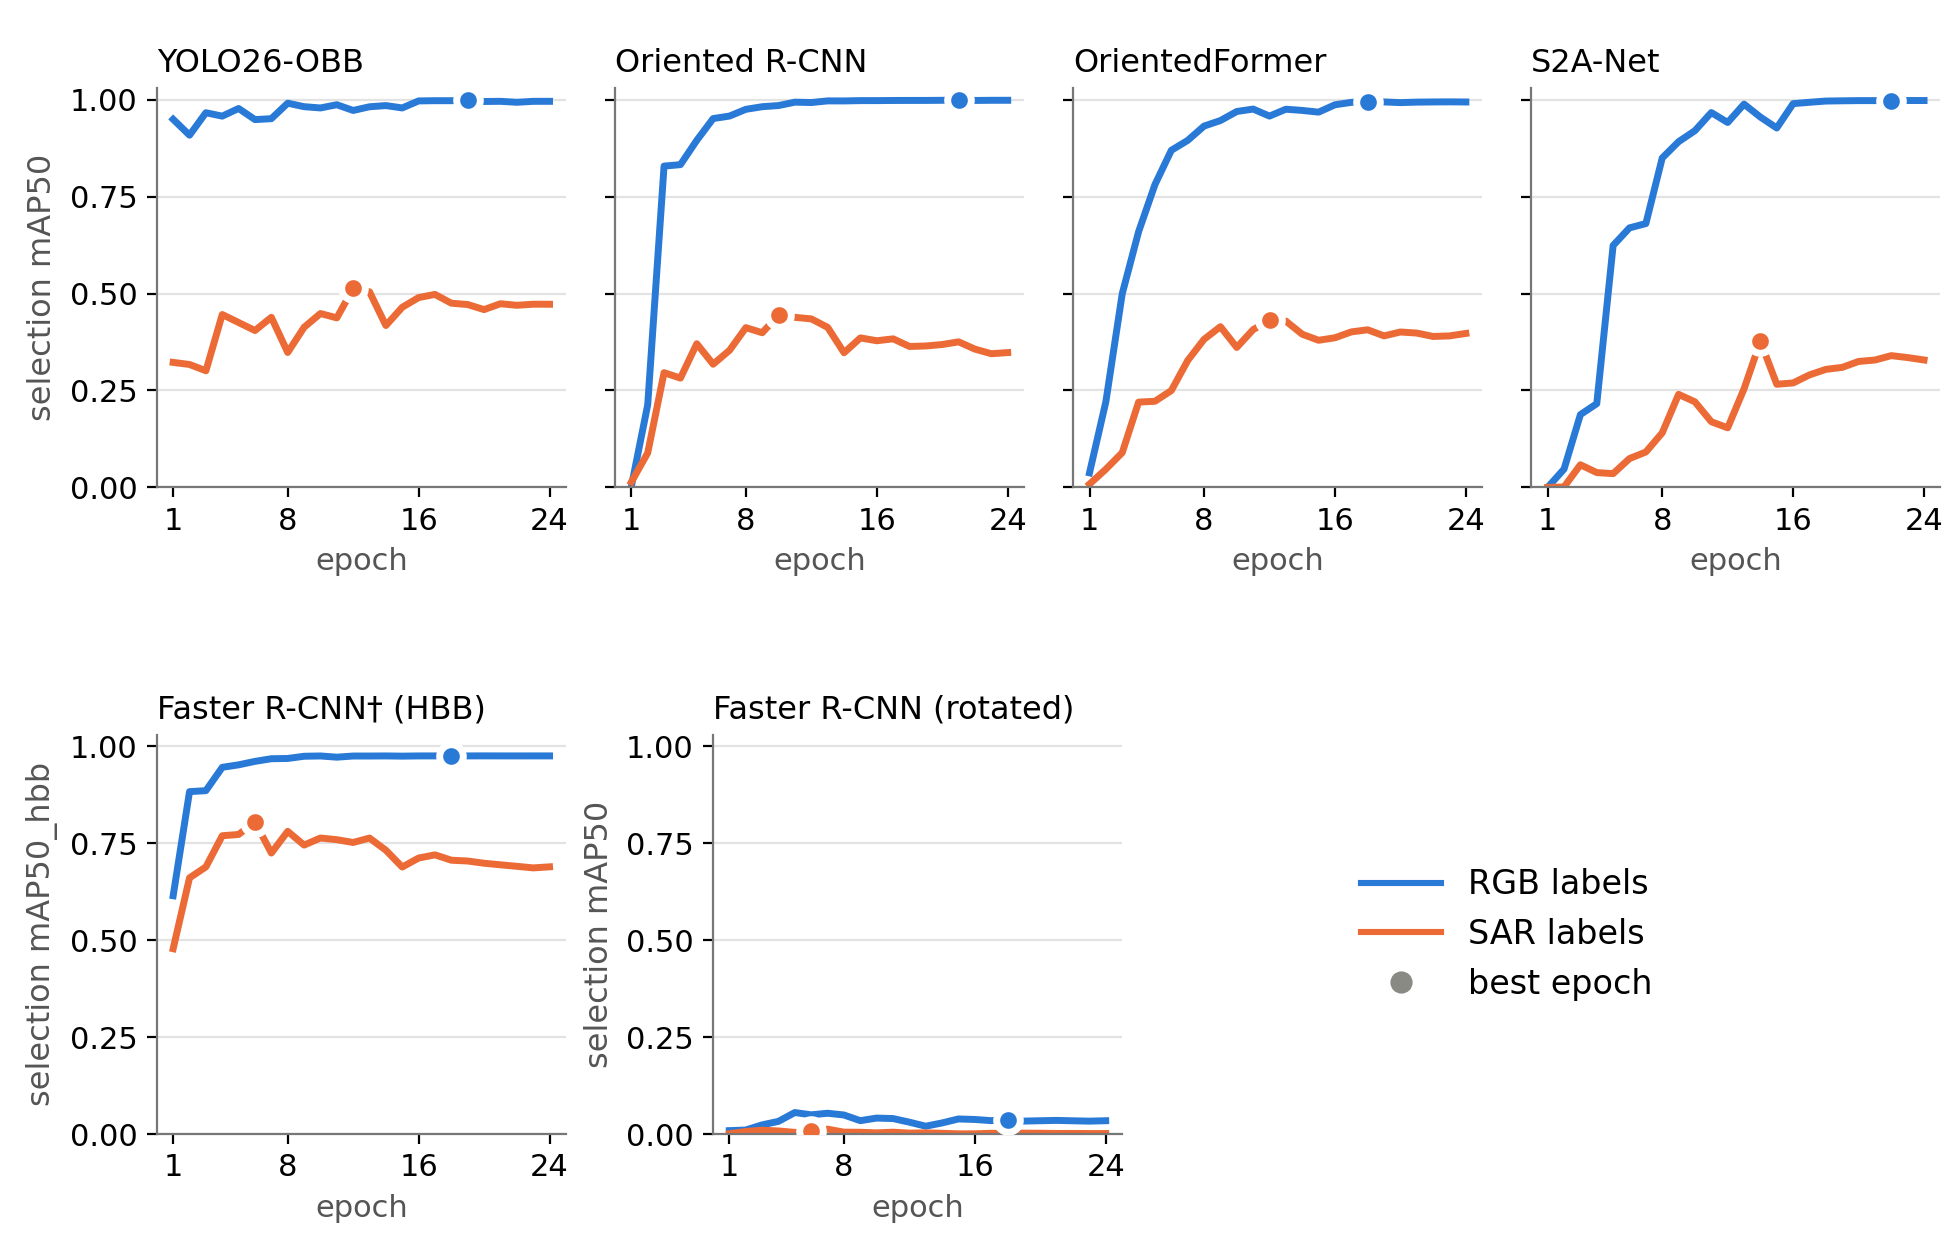
\includegraphics[width=1\textwidth]{images/selection_curves.png}
\caption{Per-epoch mAP50 on RGB and SAR labels.}
\label{fig:selection_curves}
\end{figure}


Figure~\ref{fig:selection_curves} also illustrates that SAR does not perform consistently, with results varying from 0.38 to 0.51. The peak value for the radar images occurs when the epoch ranges from 10 to 14, with scores between 0.780 and 0.953, but it begins to decline once more. In the end, we can suggest that radar images perform effectively when evaluated with the training set however they tend to fail with completely new scenes which the model has not seen before. On the other hand, examining the optical label reveals a consistent result value that is unaffected by whether or not the scenes have been previously observed.\\

\noindent\textbf{7. Analysis of the Model Dependence on Input Modalities}\\
This test checks which input each model mainly relies on, whether it uses both, and how it reacts when an input changes. First, we gave the models only the optical image, with the SAR input left blank. Next, we replaced the RGB image with a blank one and kept the SAR image. Then, we used a SAR image from another scene, so it was not aligned with the optical image. Finally, we left both inputs blank, which gave zero detections as expected.\\

\begin{figure}[htbp]
\centering
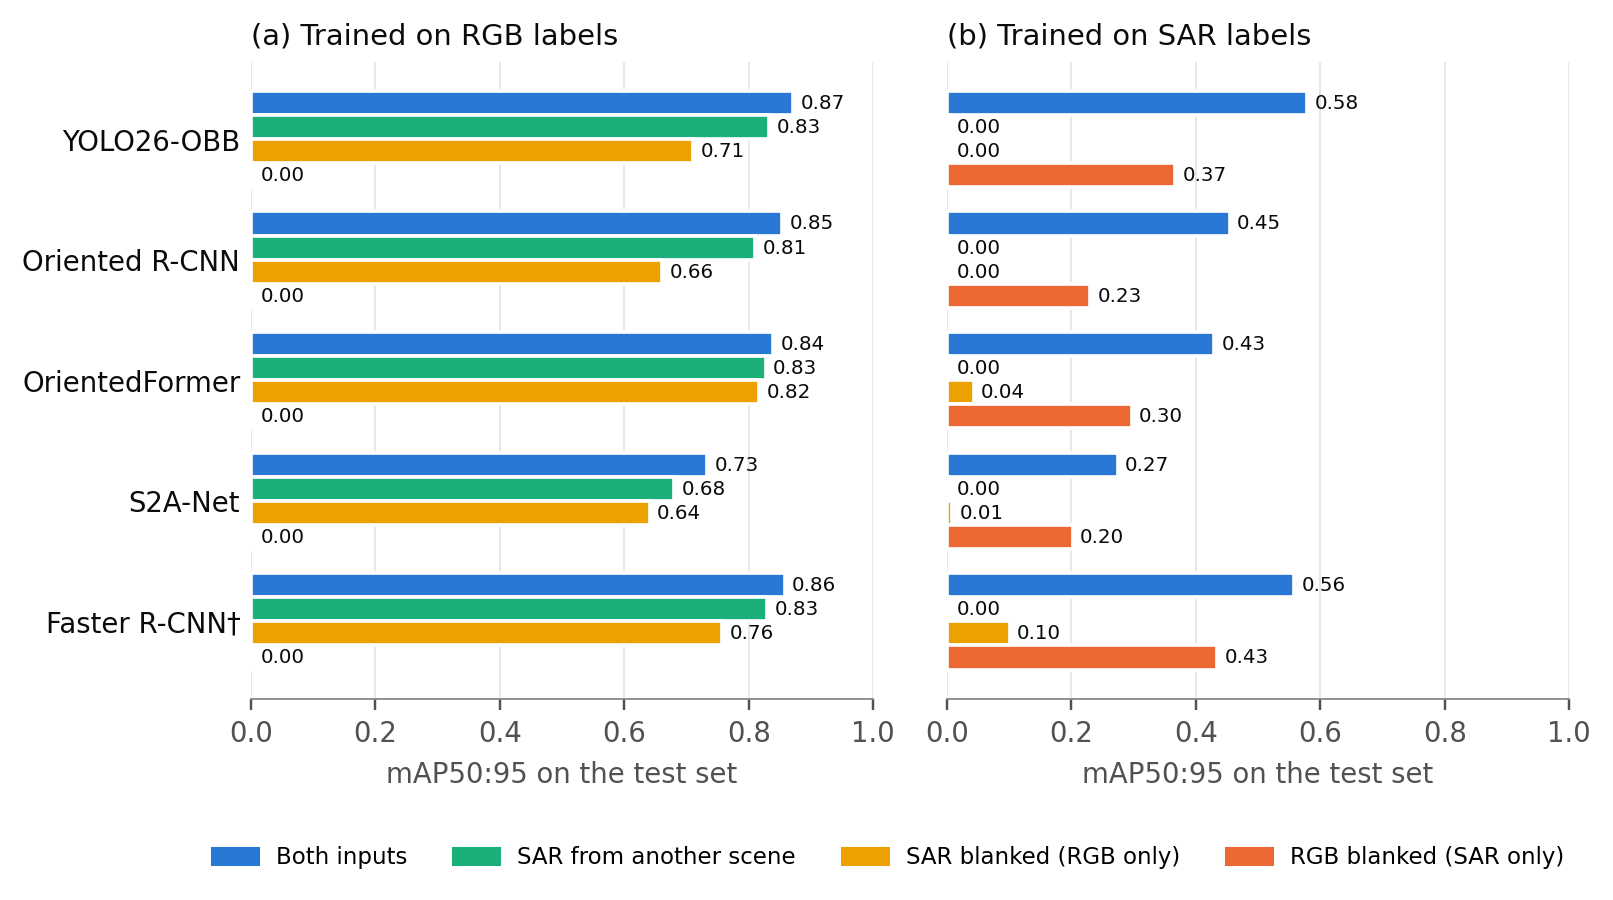
\includegraphics[width=1\textwidth]{images/modality_ablation.png}
\caption{Test time input modality ablation.}
\label{fig:modality_ablation}
\end{figure}

Figure~\ref{fig:modality_ablation} shows that the model's performance varies significantly based on its fitting; for example, an architecture optimized for SAR images will perform nearly at zero with just RGB images. We can assess this as RGB was eliminated, retaining 51 percent to 78 percent from the initial measurement. We can conclude that RGB is significant for result evaluation because it adds extra details. Currently, in RGB trained models, if optical images are omitted, it results in a score of zero; however, if we include SAR that is not aligned with optical the performance drop is only between 1.3 and 5.4 units. Nonetheless, if SAR is completely eliminated, the drop is very significant, varying from 2.3 to 19.3 units. In summary, we can state that the architectures yield optimal performance based on their calibration methods.\\

\textbf{8. Effect of SAR Input Across Ship Size}
\begin{table}[htbp]
\centering
\begin{tabular}{|l|c|c|c|c|c|c|}
\hline
 & \multicolumn{2}{c|}{\textbf{Small (214)}} & \multicolumn{2}{c|}{\textbf{Medium (762)}} & \multicolumn{2}{c|}{\textbf{Large (122)}} \\
\cline{2-7}
\textbf{Model} & \textbf{Correct} & \textbf{Shuffled} & \textbf{Correct} & \textbf{Shuffled} & \textbf{Correct} & \textbf{Shuffled} \\
\hline
YOLO26-OBB             & 0.967          & \textbf{0.944} & 0.982          & 0.932          & \textbf{1.000} & 0.836          \\
Oriented R-CNN         & 0.981          & 0.851          & 0.980          & \textbf{0.951} & 0.992          & 0.959          \\
OrientedFormer         & 0.963          & 0.921          & 0.963          & 0.944          & 0.943          & 0.861          \\
S2A-Net                & \textbf{0.991} & 0.729          & \textbf{0.992} & 0.936          & 0.951          & 0.861          \\
Faster R-CNN$^\dagger$ & 0.949          & 0.855          & 0.961          & 0.942          & 0.984          & \textbf{0.975} \\
\hline

\end{tabular}

\vspace{4pt}
\caption{Recall by Ship Size with Correct and Shuffled SAR Inputs}
\label{tab:recall_size}
\end{table}

It's an important aspect of our study on small vessel identification. Table~\ref{tab:recall_size} reports recall at IoU 0.5 and the selection-split threshold. Ships are grouped by box area into small ($< 64^2$ px), medium ($64^2$ to $128^2$ px) and large ($> 128^2$ px). As Table~\ref{tab:recall_size} shows, providing suitable radar images to architectures yields markedly better outcomes; for example, without adequate radar images, Faster R-CNN~\cite{7485869} (scored with horizontal IoU) decreased by 9.4 units, S2A-Net~\cite{han2021align} by 26.2 units, and Oriented R-CNN~\cite{xie2021oriented} fell by 13.0 units. Nonetheless, for OrientedFormer~\cite{zhao2024orientedformer} and YOLO26-OBB~\cite{jocher2026ultralytics}, the units decreased for larger scaled vessels. In the end, we can state that the score does depend on radar images, but the architecture significantly influences the benefits of using SAR images.\\

\noindent\textbf{9. Effect of Cloud Cover on Detection Performance}\\
The clouds have a minor influence in this situation since this is data generated artificially where haze or ships are lightly obscured, and typically the atmosphere tends to have greater blurriness. When the test was conducted for the YOLO26-OBB~\cite{jocher2026ultralytics} model, there was a reduction of just 0.3 when both were utilized, while removing the radar image led to a decrease of 3.4 points; however, for the other architectures, no significant changes occurred. Currently, we cannot reach a determination regarding the importance of integration or the radar imagery.\\

\noindent\textbf{10. Design Choices and Their Effect}\\
Table~\ref{tab:design_choices} lists the main design choices behind each model and how they affect the results. It helps explain why some models perform better than others on our data.

\begin{table}[htbp]
\centering

\begin{tabular}{|>{\raggedright\arraybackslash}p{5.2cm}|>{\raggedright\arraybackslash}p{8.8cm}|}
\hline
\textbf{Design choice} & \textbf{Observed effect} \\
\hline
Oriented vs horizontal boxes & Faster R-CNN~\cite{7485869} falls to 0.093 mAP50 under rotated IoU, while all oriented models stay above 0.99 \\
\hline
Full-detector DOTAv1 initialisation (YOLO26-OBB) & Best mAP50:95 with both label sources, with the fewest parameters \\
\hline
Two-stage refinement (Oriented R-CNN) vs one-stage (S2A-Net) & mAP75 of 0.985 vs 0.934 with RGB labels, even though S2A-Net has the higher recall \\
\hline
Query-based decoder trained for 24 epochs (OrientedFormer) & Lowest recall with RGB labels (43 missed ships) \\
\hline
RGB vs SAR annotations as ground truth & 29 to 46 points lower mAP50:95 with SAR labels, for every model \\
\hline
Mean-initialised $1\times1$ fusion, no modality dropout & Each model depends on the modality its labels came from; RGB-label models score zero without RGB \\
\hline
Scene-held-out selection split & Revealed that SAR-label models generalise poorly to new scenes (0.38 to 0.51 selection mAP50) \\
\hline
\end{tabular}
\caption{Design choices and the effect we observed}
\label{tab:design_choices}
\end{table}

% ============================== DISCUSSION SECTION ==============================
\section{Discussion}
\label{sec:discussion}
This study aimed to build ship detectors that fuse SAR with optical imagery, especially for small ships and ships under cloud. It also set out to understand how much each input contributes. To test this, we adapted five existing detectors so that each one takes both inputs. Then we compared them with the MOS-Ship\cite{you2026multi} with the same data split, training schedule and evaluation code. Each model's use of its RGB and SAR inputs was also studied.\\

Our results show that finding ships is not the hard part on this dataset. With RGB labels, all five detectors reach between 0.987 and 0.995 mAP50, so almost every ship is found. The models differ in how tightly they fit their boxes, which is captured by mAP50:95. YOLO26-OBB~\cite{jocher2026ultralytics} fits them the best (0.871). The model is also the smallest (33.2 M parameters) and the fastest (about 25 FPS) among all trained models for this study. Box orientation turned out to be essential. Faster R-CNN~\cite{7485869}, which predicts horizontal boxes, falls to 0.093 mAP50 once it is scored with rotated IoU, because a horizontal box around a diagonal ship also covers the sea and the ships next to it.\\

The label source mattered more than the choice of model. The RGB and SAR annotations of the same ship match at a median IoU of only 0.458. Training on SAR labels cost every model between 29 and 46 points of mAP50:95. The SAR-label models also generalised poorly to unseen scenes, with selection mAP50 stuck between 0.38 and 0.51.\\

The most important finding came from a test-time ablation. Here, the fused models were not retrained. Instead, at test time we either blanked one input, so the model saw only RGB or only SAR, or replaced the SAR tile with the SAR image of a tile from another scene. When we replaced the SAR tile with SAR from another scene, every RGB-label model lost 1.3 to 5.4 points of mAP50:95. From that result we can claim that the fused models do use the SAR content, not just its presence. In three of the five models, aligned SAR mattered most for small ships. But each model mostly depended on the image from where its annotations came from. Without that image, it found few or no ships. Models trained on RGB labels scored zero once the RGB image was removed. This is the situation where SAR should take over, for example under thick clouds or at night. These tests change the inputs of a fused model at test time. They show what each model relies on, but they don't tell us whether fusion beats a detector trained on one input alone. That needs RGB-only and SAR-only models trained with the same setup. The official cloud tiles couldn't test robustness either, because they leave most ships visible and cost the fused models at most 1.5 points.\\

Our results cannot be compared directly with the MOS-Ship paper, which reports 84.1 AP50 for MOS-DETR \cite{you2026multi}. Its model reads one image at a time and fuses the detections only at the end, and the paper does not state which annotations its test sets are scored against.\\

\noindent\textbf{Key Achievements:}
\begin{itemize}
    \item Five dual-stream detectors were built in one code base and compared fairly.
    \item Checkpoints and test thresholds were chosen on a scene-held-out split.
    \item YOLO26-OBB~\cite{jocher2026ultralytics} was selected as the best model, leading on accuracy, size and speed.
    \item We showed that the fused models use SAR content, and that aligned SAR helps small-ship detection in three of the five models.
    \item We found that the mismatch between RGB and SAR labels is the main reason our results differ from the MOS-Ship paper\cite{you2026multi}.
\end{itemize}



